% PRISMA-trAIce flow diagram, landscape (slide) version
% Same content as Figure 1 in LitReview_Flowchart.tex, re-laid out left-to-right
% so it fits under a title on a 16:9 PowerPoint slide.
% Compile: pdflatex LitReview_Flowchart_Landscape.tex
%%%%%%%%%%%%%%%%%%%%%%%%%%%%%%%%%%%%%%%%%%%%%%%%%%%%%%%%%%%%%%%%%%%
\documentclass[border=6pt]{standalone}
\usepackage[T1]{fontenc}
\usepackage[scaled=0.95]{helvet}
\renewcommand{\familydefault}{\sfdefault}
\usepackage{amssymb}
\usepackage{xcolor}
\usepackage{array}
\usepackage{tikz}
\usetikzlibrary{arrows.meta, positioning, calc, fit, backgrounds}

% Counts. Change \numcolor to red to flag provisional numbers again.
\colorlet{numcolor}{black}
\newcommand{\n}[1]{\textbf{\textcolor{numcolor}{#1}}}
\newcommand{\tbd}[1]{\textbf{\textcolor{red}{#1}}}
% Exclusion reason rows: reason left, count right
\newcommand{\rsn}[2]{#1 & \n{#2}\\}
\newenvironment{reasons}[1]
  {\footnotesize\renewcommand{\arraystretch}{1.05}%
   \begin{tabular}{@{}>{\raggedright\arraybackslash}p{#1}@{\hspace{3pt}}r@{}}}
  {\end{tabular}}

% No hyphenation inside boxes
\hyphenpenalty=10000 \exhyphenpenalty=10000

\begin{document}
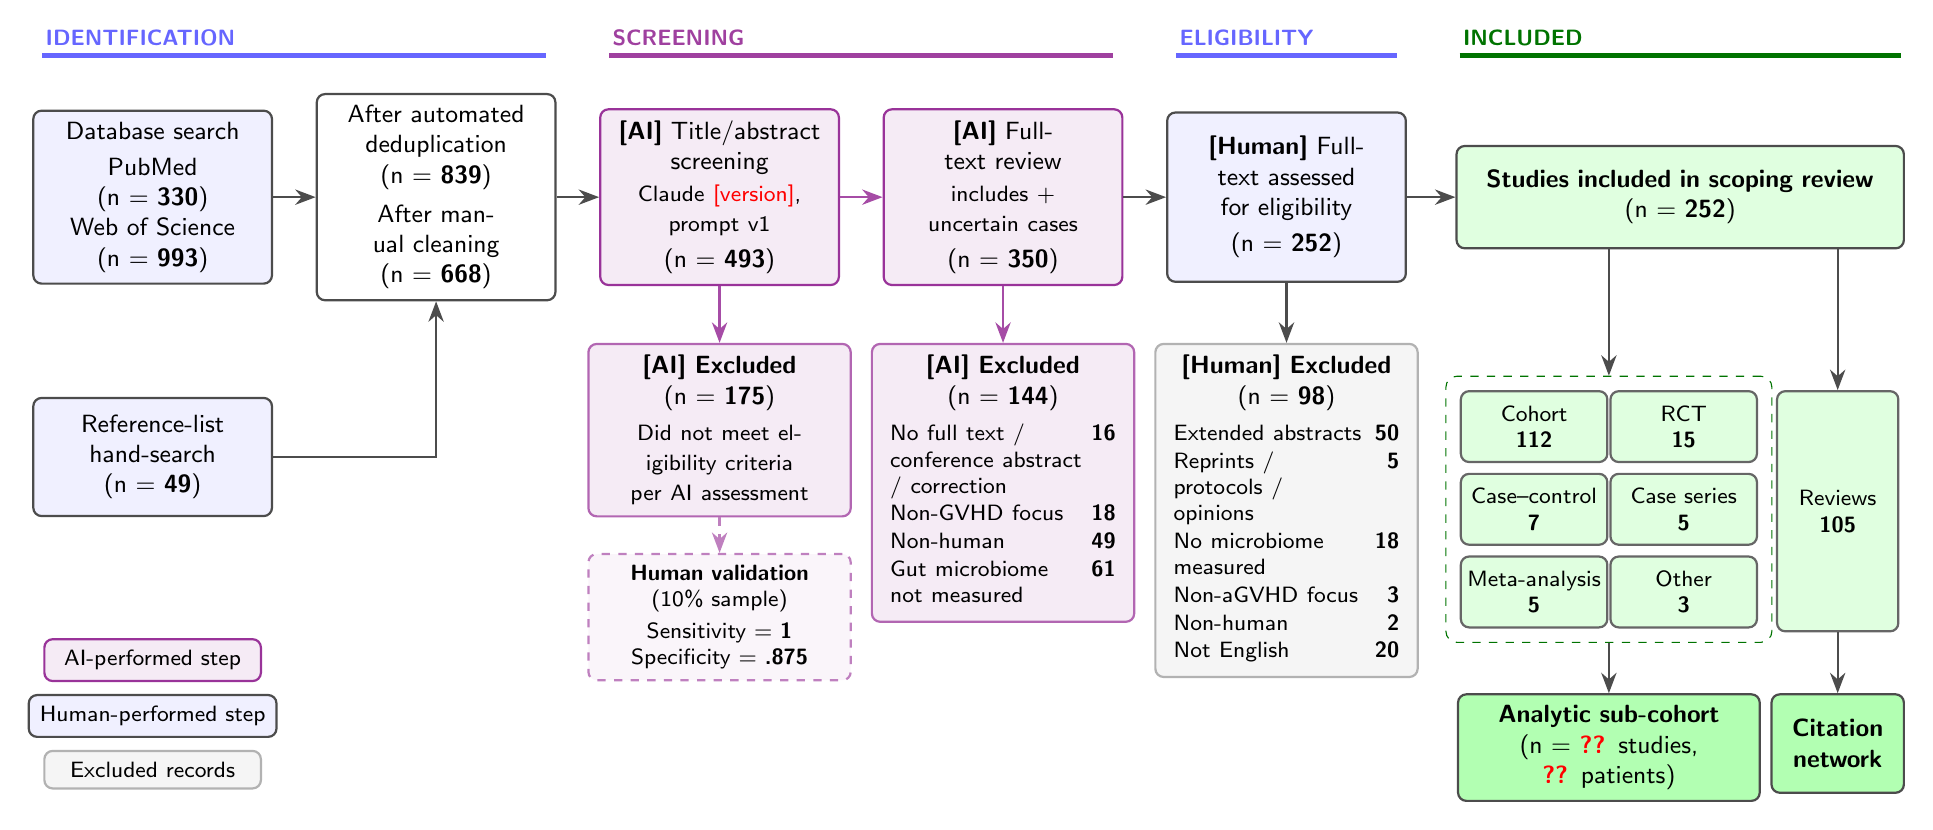
\begin{tikzpicture}[
    font=\small,
    base/.style={rectangle, thick, rounded corners=3pt, align=center,
                 inner sep=4pt},
    box/.style={base, draw=black!70, fill=blue!6, text width=2.75cm,
                minimum height=2.15cm},
    aibox/.style={base, draw=violet!80, fill=violet!8, text width=2.75cm,
                  minimum height=2.15cm},
    excbox/.style={base, draw=gray!60, fill=gray!8, text width=3.05cm,
                   anchor=north},
    aiexcbox/.style={base, draw=violet!60, fill=violet!8, text width=3.05cm,
                     anchor=north},
    notebox/.style={base, draw=violet!50, dashed, fill=violet!4,
                    text width=3.05cm, font=\footnotesize, anchor=north},
    inclbox/.style={base, draw=black!70, fill=green!12},
    catbox/.style={base, draw=black!60, fill=green!12, text width=1.72cm,
                   minimum height=0.9cm, inner sep=2pt, font=\footnotesize},
    resultbox/.style={base, draw=black!70, fill=green!30, minimum height=1.25cm},
    arrow/.style={-{Stealth[length=2.6mm]}, thick, black!70},
    aiarrow/.style={-{Stealth[length=2.6mm]}, thick, violet!70},
    phase/.style={font=\footnotesize\bfseries, anchor=south west, inner sep=1pt},
]

%-------- COLUMN CENTRES --------
\def\cA{1.55}  \def\cB{5.15}  \def\cC{8.75}
\def\cD{12.35} \def\cE{15.95}
\def\yMain{10.2}

%-------- PHASE HEADERS --------
\foreach \xa/\xb/\lab/\col in {0.15/6.55/Identification/blue!60,
                               7.35/13.75/Screening/violet!75,
                               14.55/17.35/Eligibility/blue!60,
                               18.15/23.75/Included/green!45!black}{
  \draw[\col, line width=1.6pt] (\xa,12.0) -- (\xb,12.0);
  \node[phase, text=\col] at (\xa,12.08) {\MakeUppercase{\lab}};
}

%-------- IDENTIFICATION --------
\node[box] (db) at (\cA,\yMain)
  {Database search\\[2pt]PubMed\\(n~=~\n{330})\\Web of Science\\(n~=~\n{993})};
\node[box, minimum height=1.5cm] (hand) at (\cA,6.9)
  {Reference-list\\hand-search\\(n~=~\n{49})};
\node[box, fill=white] (dedup) at (\cB,\yMain)
  {After automated deduplication\\(n~=~\n{839})\\[3pt]After manual cleaning\\(n~=~\n{668})};

%-------- SCREENING (AI) --------
\node[aibox] (aiscreen) at (\cC,\yMain)
  {\textbf{[AI]} Title/abstract screening\\[2pt]
   {\footnotesize Claude \textcolor{red}{[version]},\\prompt v1}\\[2pt]
   (n~=~\n{493})};
\node[aiexcbox] (aiexcl) at (\cC,8.35)
  {\textbf{[AI] Excluded}\\(n~=~\n{175})\\[2pt]
   {\footnotesize Did not meet eligibility criteria per AI assessment}};
\node[notebox, below=0.45cm of aiexcl] (aiperf)
  {\textbf{Human validation}\\(10\% sample)\\[2pt]
   Sensitivity~=~\n{1}\\Specificity~=~\n{.875}};

\node[aibox] (aift) at (\cD,\yMain)
  {\textbf{[AI]} Full-text review\\[2pt]
   {\footnotesize includes +\\uncertain cases}\\[2pt]
   (n~=~\n{350})};
\node[aiexcbox] (aiftexcl) at (\cD,8.35)
  {\textbf{[AI] Excluded}\\(n~=~\n{144})\\[3pt]
   \begin{reasons}{2.45cm}
   \rsn{No full text / conference abstract / correction}{16}
   \rsn{Non-GVHD focus}{18}
   \rsn{Non-human}{49}
   \rsn{Gut microbiome not measured}{61}
   \end{reasons}};

%-------- ELIGIBILITY (HUMAN) --------
\node[box] (elig) at (\cE,\yMain)
  {\textbf{[Human]} Full-text assessed for eligibility\\[2pt](n~=~\n{252})};
\node[excbox] (humexcl) at (\cE,8.35)
  {\textbf{[Human] Excluded}\\(n~=~\n{98})\\[3pt]
   \begin{reasons}{2.45cm}
   \rsn{Extended abstracts}{50}
   \rsn{Reprints / protocols / opinions}{5}
   \rsn{No microbiome measured}{18}
   \rsn{Non-aGVHD focus}{3}
   \rsn{Non-human}{2}
   \rsn{Not English}{20}
   \end{reasons}};

%-------- INCLUDED --------
\node[inclbox, text width=5.4cm, minimum height=1.3cm] (incl) at (20.95,\yMain)
  {\textbf{Studies included in scoping review}\\(n~=~\n{252})};

% Study-design categories: six designs feeding the analytic sub-cohort (2 x 3 grid)
\def\gx{18.15} \def\gy{7.75}
\node[catbox, anchor=north west] (coh)  at (\gx,\gy)          {Cohort\\\n{112}};
\node[catbox, anchor=north west] (rct)  at (\gx+1.9,\gy)      {RCT\\\n{15}};
\node[catbox, anchor=north west] (cc)   at (\gx,\gy-1.05)     {Case--control\\\n{7}};
\node[catbox, anchor=north west] (cs)   at (\gx+1.9,\gy-1.05) {Case series\\\n{5}};
\node[catbox, anchor=north west] (meta) at (\gx,\gy-2.1)      {Meta-analysis\\\n{5}};
\node[catbox, anchor=north west] (oth)  at (\gx+1.9,\gy-2.1)  {Other\\\n{3}};
\begin{scope}[on background layer]
  \node[draw=green!45!black, dashed, rounded corners=4pt, inner sep=5pt,
        fit=(coh)(oth)] (grp) {};
\end{scope}
\node[catbox, text width=1.4cm, minimum height=3.05cm, anchor=north]
  (rev) at (22.95,\gy) {Reviews\\\n{105}};

\node[resultbox, text width=3.55cm, anchor=north] (sub) at (grp.south |- 0,3.9)
  {\textbf{Analytic sub-cohort}\\(n~=~\tbd{??} studies,\\\tbd{??} patients)};
\node[resultbox, text width=1.4cm, anchor=north] (cite) at (rev.south |- 0,3.9)
  {\textbf{Citation network}};

%-------- ARROWS: main flow --------
\draw[arrow]   (db)       -- (dedup);
\draw[arrow]   (hand.east) -| (dedup.south);
\draw[arrow]   (dedup)    -- (aiscreen);
\draw[aiarrow] (aiscreen) -- (aift);
\draw[arrow]   (aift)     -- (elig);
\draw[arrow]   (elig)     -- (incl);

%-------- ARROWS: exclusions --------
\draw[aiarrow] (aiscreen) -- (aiexcl);
\draw[arrow, violet!50, dashed] (aiexcl) -- (aiperf);
\draw[aiarrow] (aift)     -- (aiftexcl);
\draw[arrow]   (elig)     -- (humexcl);

%-------- ARROWS: included -> designs -> downstream --------
\draw[arrow] (incl.south -| grp.north) -- (grp.north);
\draw[arrow] (incl.south -| rev.north) -- (rev.north);
\draw[arrow] (grp.south) -- (sub.north);
\draw[arrow] (rev.south) -- (cite.north);

%-------- LEGEND --------
\node[base, draw=violet!80, fill=violet!8, font=\footnotesize, minimum width=2.75cm,
      anchor=north] (legai) at (\cA,4.6) {AI-performed step};
\node[base, draw=black!70, fill=blue!6, font=\footnotesize, minimum width=2.75cm,
      below=0.15cm of legai] (leghu) {Human-performed step};
\node[base, draw=gray!60, fill=gray!8, font=\footnotesize, minimum width=2.75cm,
      below=0.15cm of leghu] {Excluded records};

\end{tikzpicture}
\end{document}
